\documentclass[fleqn, a4paper, 12pt, twoside]{article}
\usepackage{exsheets}
\usepackage{amsmath, amssymb, amsthm} %standard AMS packages
\usepackage{marginnote} %marginnotes
\usepackage{gensymb} %miscellaneous symbols
\usepackage{commath} %differential symbols
\usepackage{xcolor} %colours
\usepackage{cancel} %cancelling terms
\usepackage[free-standing-units]{siunitx} %formatting units
\usepackage{tikz, pgfplots} %diagrams
	\usetikzlibrary{calc, hobby, patterns, intersections}
\usepackage{graphicx} %inserting graphics
\usepackage{hyperref} %hyperlinks
\usepackage{datetime} %date and time
\usepackage{ulem} %underline for \emph{}
\usepackage{xfrac, lmodern} %inline fractions
\usepackage{enumerate, enumitem} %numbered lists
\usepackage{float} %inserting floats
\usepackage{tabularx}

\newcommand\numberthis{\addtocounter{equation}{1}\tag{\theequation}} %adds numbers to specific equations in non-numbered list of equations

\newcommand{\AxisRotator}[1][rotate=0]{
	\tikz [x=0.25cm,y=0.60cm,line width=.2ex,-stealth,#1] \draw (0,0) arc (-150:150:1 and 1);%
} %rotation symbols on axes

\theoremstyle{definition}
\newtheorem{example}{Example}
\newtheorem{definition}{Definition}

\theoremstyle{theorem}
\newtheorem{theorem}{Theorem}

\newcommand{\curl}{\mathrm{curl\,}}

\newcommand{\divergence}{\mathrm{div\,}}

\makeatletter
\@addtoreset{section}{part} %resets section numbers in new part
\makeatother

\makeatletter
\newcommand*{\relrelbarsep}{.386ex}
\newcommand*{\relrelbar}{%
  \mathrel{%
    \mathpalette\@relrelbar\relrelbarsep
  }%
}
\newcommand*{\@relrelbar}[2]{%
  \raise#2\hbox to 0pt{$\m@th#1\relbar$\hss}%
  \lower#2\hbox{$\m@th#1\relbar$}%
}
\providecommand*{\rightrightarrowsfill@}{%
  \arrowfill@\relrelbar\relrelbar\rightrightarrows
}
\providecommand*{\leftleftarrowsfill@}{%
  \arrowfill@\leftleftarrows\relrelbar\relrelbar
}
\providecommand*{\xrightrightarrows}[2][]{%
  \ext@arrow 0359\rightrightarrowsfill@{#1}{#2}%
}
\providecommand*{\xleftleftarrows}[2][]{%
  \ext@arrow 3095\leftleftarrowsfill@{#1}{#2}%
}
\makeatother

\newcommand\blfootnote[1]{%
	\begingroup
	\renewcommand\thefootnote{}\footnote{#1}%
	\addtocounter{footnote}{-1}%
	\endgroup
}

\SetupExSheets{solution/print = true} %prints all solutions by default
%opening
\title{Differential and Integral Calculus\\Review Session}
\author{Aakash Jog}
\date{\formatdate{17}{6}{2015}}

\begin{document}

\maketitle
%\setlength{\mathindent}{0pt}

\blfootnote
{	
	\begin{figure}[H]
		
\includegraphics[height = 12pt]{cc.eps}
		\includegraphics[height = 12pt]{by.eps}
		\includegraphics[height = 12pt]{nc.eps}
		\includegraphics[height = 12pt]{sa.eps}
	\end{figure}
	This work is licensed under the Creative Commons Attribution-NonCommercial-ShareAlike 4.0 International License. To view a copy of this license, visit \url{http://creativecommons.org/licenses/by-nc-sa/4.0/}.
} %CC-BY-NC-SA licencse

\newpage
\begin{question}
	Does the sequence of functions
	\begin{align*}
		f_n(x) & = \frac{x^2}{x^2 + (n x - 1)^2}
	\end{align*}
	converge uniformly on $[0,1]$?
\end{question}

\begin{solution}
	$\forall x \in [0,1]$,
	\begin{align*}
		\lim\limits_{n \to \infty} \frac{x^2}{x^2 + (n x - 1)^2} & = 0
	\end{align*}
	Therefore, $f_n(x)$ converges pointwise to $f(x) = 0$ in $[0,1]$.\\
	\begin{align*}
		\lim\limits_{n \to \infty} \sup\limits_{[0,1]} \left| f_n(x) - f(x) \right| & = \lim\limits_{n - \infty} \sup\limits_{[0,1]} \frac{x^2}{x^2 + (n x - 1)^2}
	\end{align*}
	As the function is continuous on the interval,
	\begin{align*}
		\sup\limits_{[0,1]} \frac{x^2}{x^2 + (n x - 1)^2} & = \max\limits_{[0,1]} \frac{x^2}{x^2 + (n x - 1)^2}
	\end{align*}
	Therefore, differentiating to find critical points,
	\begin{align*}
		{f_n}'(x) & = \frac{2 x \left( x^2 + (n x - 1)^2 \right) - x^2 \left( 2 x + 2 (n x - 1) n \right)}{\left( x^2 + (n x - 1)^2 \right)^2} \\
                          & = \frac{2 x (n x - 1)^2 - 2 n x^2 (n x - 1)}{\left( x^2 + (n x - 1)^2 \right)^2}                                           \\
                          & = \frac{2 x (n x - 1) (n x - 1 - n x)}{\left( x^2 + (n x - 1)^2 \right)^2}                                                 \\
                          & = \frac{-2 x (n x - 1)}{\left( x^2 + (n x - 1)^2 \right)^2}                                                                \\
                          & = \frac{2 x (1 - n x)}{\left( x^2 + (n x - 1)^2 \right)^2}
	\end{align*}
	Therefore, the function has critical points at $x = 0$ and $x = \frac{1}{n}$.\\
	Therefore, checking the critical points and the end-points,
	\begin{align*}
		f_n(0)                        & = 0                                       \\
		f_n(1)                        & = \frac{1}{1 + (n - 1)^2}                 \\
		f_n\left( \frac{1}{n} \right) & = \frac{\frac{1}{n^2}}{\frac{1}{n^2} + 0} \\
                                              & = 1
	\end{align*}
	Therefore,
	\begin{align*}
		\sup\limits_{[0,1]} \frac{x^2}{x^2 + (n x - 1)^2} & = \max\limits_{[0,1]} \frac{x^2}{x^2 + (n x - 1)^2} \\
                                                                  & = 1
	\end{align*}
	Therefore,
	\begin{align*}
		\lim\limits_{n \to \infty} \sup\limits_{[0,1]} \frac{x^2}{x^2 + (n x - 1)^2} & = 1
	\end{align*}
	Therefore, as $\lim\limits_{n \to \infty} \left| f_n(x) - f(x) \right| \neq 0$, the sequence does not converge uniformly on $[0,1]$.
\end{solution}

\begin{question}
	Given $a,b > 0$, calculate the double integral $\iint\limits_{D} x y \dif A$, where $D$ is a quarter of the ellipse given by $\frac{x^2}{a^2} + \frac{y^2}{b^2} \le 1$, for $x \ge 0$, $y \ge 0$.
\end{question}

\begin{solution}
	Let
	\begin{align*}
		x & = a r \cos \theta \\
		y & = b r \sin \theta
	\end{align*}
	Therefore,
	\begin{align*}
		J &=
			\begin{vmatrix}
				x_r & x_{\theta} \\
				y_r & y_{\theta} \\
			\end{vmatrix}\\
		  &=
			\begin{vmatrix}
				a \cos \theta & -a r \sin \theta \\
				b \sin \theta & b r \cos \theta  \\
			\end{vmatrix}\\
		  &= a b r
	\end{align*}
	Therefore,
	\begin{align*}
		\iint\limits_{D} x y \dif A & = \int\limits_{0}^{1} \int\limits_{0}^{\frac{\pi}{2}} a r \cos \theta \cdot b r \sin \theta \cdot a b r \dif \theta \dif r \\
                                            & = a^2 b^2 \int\limits_{0}^{1} r^3 \dif r \int\limits_{0}^{\frac{\pi}{2}} \cos \theta \sin \theta \dif \theta               \\
                                            & = \frac{1}{8} a^2 b^2
	\end{align*}
\end{solution}

\begin{question}
	Check if the following series converge conditionally, converge absolutely, or diverge.
	\begin{enumerate}
		\item $\displaystyle \sum\limits_{n = 1}^{\infty} (-1)^n \sin^3 \frac{1}{\sqrt{n}}$
		\item $\displaystyle \sum\limits_{n = 1}^{\infty} \frac{n!}{n^{\frac{n}{2}}}$
	\end{enumerate}
\end{question}

\begin{solution}
	\begin{enumerate}[leftmargin = *]
		\item
			\begin{align*}
				\left| (-1)^n \sin^3 \frac{1}{\sqrt{n}} \right| & = \sin^3 \frac{1}{\sqrt{n}}                 \\
                                                                                & \approx \left( \frac{1}{\sqrt{n}} \right)^3 \\
                                                                                & = \frac{1}{n^{\frac{3}{2}}}
			\end{align*}
			Therefore, as $\sum \frac{1}{n^{\frac{3}{2}}}$ converges, the series converges absolutely.
		\item
			\begin{align*}
				a_n & = \frac{n!}{n^{\frac{n}{2}}}
			\end{align*}
			Therefore,
			\begin{align*}
				\left| \frac{a_{n + 1}}{a_n} \right| & = \frac{\frac{n!}{n^{\frac{n}{2}}}}{\frac{(n + 1)!}{(n + 1)^{\frac{n + 1}{2}}}} \\
                                                                     & = \frac{(n + 1) n^{\frac{n}{2}}}{(n + 1)^{\frac{1}{2}} (n + 1)^{\frac{n}{2}}}   \\
                                                                     & = \sqrt{n + 1} \frac{1}{\left( \frac{n + 1}{n} \right)^{\frac{n}{2}}}           \\
                                                                     & = \sqrt{n + 1} \frac{1}{\left( \left( 1 + \frac{1}{n} \right)^n \right)^{\frac{1}{2}}}
			\end{align*}
			Therefore,
			\begin{align*}
				\lim\limits_{n \to \infty} \left| \frac{a_{n + 1}}{a_n} \right| & = \lim\limits_{n \to \infty} \sqrt{n + 1} \frac{1}{\left( \left( 1 + \frac{1}{n} \right)^n \right)^{\frac{1}{2}}} \\
                                                                                                & = \infty                                                                                                          \\
                                                                                                & > 1
			\end{align*}
			Therefore, by the ratio test, the series diverges.
	\end{enumerate}
\end{solution}

\begin{question}
	Calculate the volume of the body which is bounded by a cone $z = \sqrt{x^2 + y^2}$ and the cylinder $x^2 + y^2 = x$ with $z \ge 0$.
\end{question}

\begin{solution}
	\begin{align*}
		x^2 + y^2                                         & = x \\
		\therefore \left( x - \frac{1}{2} \right)^2 + y^2 & = \frac{1}{4}
	\end{align*}
	Therefore, the cylinder is centred at $\left( \frac{1}{2} , 0 \right)$, and has radius $\frac{1}{2}$.\\
	Therefore, the volume of the body is
	\begin{align*}
		\iiint\limits_{E_{\mathrm{I}}} \dif V \\
                                                       & = \iint\limits_{D} \int\limits_{0}^{\sqrt{x^2 + y^2}} \dif z \dif A \\
                                                       & = \iint\limits_{D} \sqrt{x^2 + y^2} \dif A
	\end{align*}
	Let
	\begin{align*}
		x & = r \cos \theta \\
		y & = r \sin \theta
	\end{align*}
	Therefore, the $D$ is given by $-\frac{\pi}{2} \le \theta \frac{\pi}{2}$ and $0 \le r \le \cos \theta$.\\
	Therefore,
	\begin{align*}
		\iint\limits_{E_{\mathrm{I}}} \dif V & = \iint\limits_{D} \sqrt{x^2 + y^2} \dif A                                                                       \\
                                                     & = \int\limits_{-\frac{\pi}{2}}^{\frac{\pi}{2}} \int\limits_{0}^{\cos \theta} r \cdot r \dif r \dif \theta        \\
                                                     & = \int\limits_{-\frac{\pi}{2}}^{\frac{\pi}{2}} \left. \frac{r^3}{3} \right|_{0}^{\cos \theta} \dif \theta        \\
                                                     & = \frac{1}{3} \int\limits_{-\frac{\pi}{2}}^{\frac{\pi}{2}} \cos^3 \theta \dif \theta                             \\
                                                     & = \frac{2}{3} \int\limits_{0}^{\frac{\pi}{2}} \cos^3 \theta \dif \theta                                          \\
                                                     & = \frac{2}{3} \int\limits_{0}^{\frac{\pi}{2}} \cos^2 \theta \cos \theta \dif \theta                              \\
                                                     & = \frac{2}{3} \int\limits_{0}^{\frac{\pi}{2}} \left( 1 - \sin^2 \theta \right) \cos \theta \dif \theta           \\
                                                     & = \frac{2}{3} \int\limits_{0}^{\frac{\pi}{2}} \left( \cos \theta - \sin^2 \theta \cos \theta \right) \dif \theta \\
                                                     & = \frac{4}{9}
	\end{align*}
\end{solution}

\end{document}
